\begin{figure}[ht]
  \centering
  \begin{subfigure}[b]{0.4\textwidth}
    \centering
    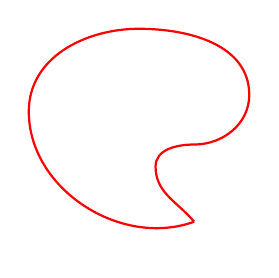
\begin{tikzpicture}[scale=0.7]
      \draw[red,thick] (1,0) to [out=200,in=270] (-2,2)
      to [out=90,in=180] (0,3.5)
      to [out=0,in=90] (2,2.3)
      to [out=270,in=0] (1,1.4)
      to [out=180,in=90] (0.3,1)
      to [out=270,in=130] (1,0);
    \end{tikzpicture}
    \caption{Simple}
  \end{subfigure}
  \hspace{1cm}
  \begin{subfigure}[b]{0.4\textwidth}
    \centering
    
\begin{tikzpicture}[scale=0.7]
      \draw[red,thick] (0,0) to [out=90,in=180] (1.5,2)
      to [out=0,in=30] (0,0) 
      to [out=210,in=180] (-1.5,-2)
      to [out=0,in=270] (0,0);
    \end{tikzpicture}
    \caption{No simple}
    \label{fig:trayectoria_nosimple}
  \end{subfigure}
  \caption{Trayectorias cerradas}
\end{figure}
